\section{Experimental Results}

\subsection{Prediction Performance}
Table~\ref{tab:pred_perf} summarizes macro performance across compared models in the multimodal task. Random Forest achieved the lowest average error, while the SNN remained competitive and more stable than a simple MLP baseline.

\begin{table}[!h]
\caption{Multimodal prediction performance (macro metrics).}
\label{tab:pred_perf}
\centering
\begin{tabular}{lccc}
\toprule
Model & MAE & RMSE & $R^2$ \\
\midrule
Random Forest & 0.438 & 0.572 & 0.350 \\
LSTM & 0.455 & 0.593 & 0.322 \\
SNN (proposed) & 0.483 & 0.617 & 0.256 \\
MLP & 0.560 & 0.694 & 0.180 \\
\bottomrule
\end{tabular}
\end{table}

The numerical ranking indicates that Random Forest achieves the lowest MAE, while the proposed SNN remains in a competitive range and preserves the edge-oriented advantages discussed in this paper, especially when considering deployment constraints beyond pure predictive accuracy.

\subsection{Energy Consumption and Latency}
Table~\ref{tab:energy_latency} reports incremental energy-per-inference and throughput across deployment platforms. ESP32 is feasible for low-rate autonomous scenarios but has higher energy per inference due to limited throughput. Raspberry Pi and Android devices provide much lower mJ/inf in high-throughput settings.

\begin{table}[!htbp]
\caption{Latency/throughput and incremental energy across platforms.}
\label{tab:energy_latency}
\centering
\begin{tabular}{lccc}
\toprule
Platform & Throughput (samples/s) & $\Delta P$ (W) & Energy (mJ/inf) \\
\midrule
ESP32 (MicroPython) & 5.0 & 0.056 & 11.204 \\
Raspberry Pi 4B & 4670.50 & 0.239 & 0.0512 \\
Device A (Android) & 12337.40 & 0.128 & 0.0104 \\
Device B (Android) & 30905.08 & 0.468 & 0.0151 \\
Device C (Android) & 16121.71 & 0.046 & 0.00285 \\
\bottomrule
\end{tabular}
\end{table}

Figure~\ref{fig:energy_bar_lnncs} compares the incremental energy per inference across deployment platforms using a logarithmic scale to preserve visual readability despite large magnitude differences. The plot shows that ESP32 has the highest energy cost per prediction, mainly due to its low throughput, while Raspberry Pi and Android devices operate in a much lower mJ/inf range. Among mobile platforms, the figure also highlights that higher throughput does not always imply lower energy per inference, reinforcing that platform selection should be based on the joint analysis of processing speed and incremental power behavior under real deployment conditions.

\begin{figure}[!htbp]
\centering
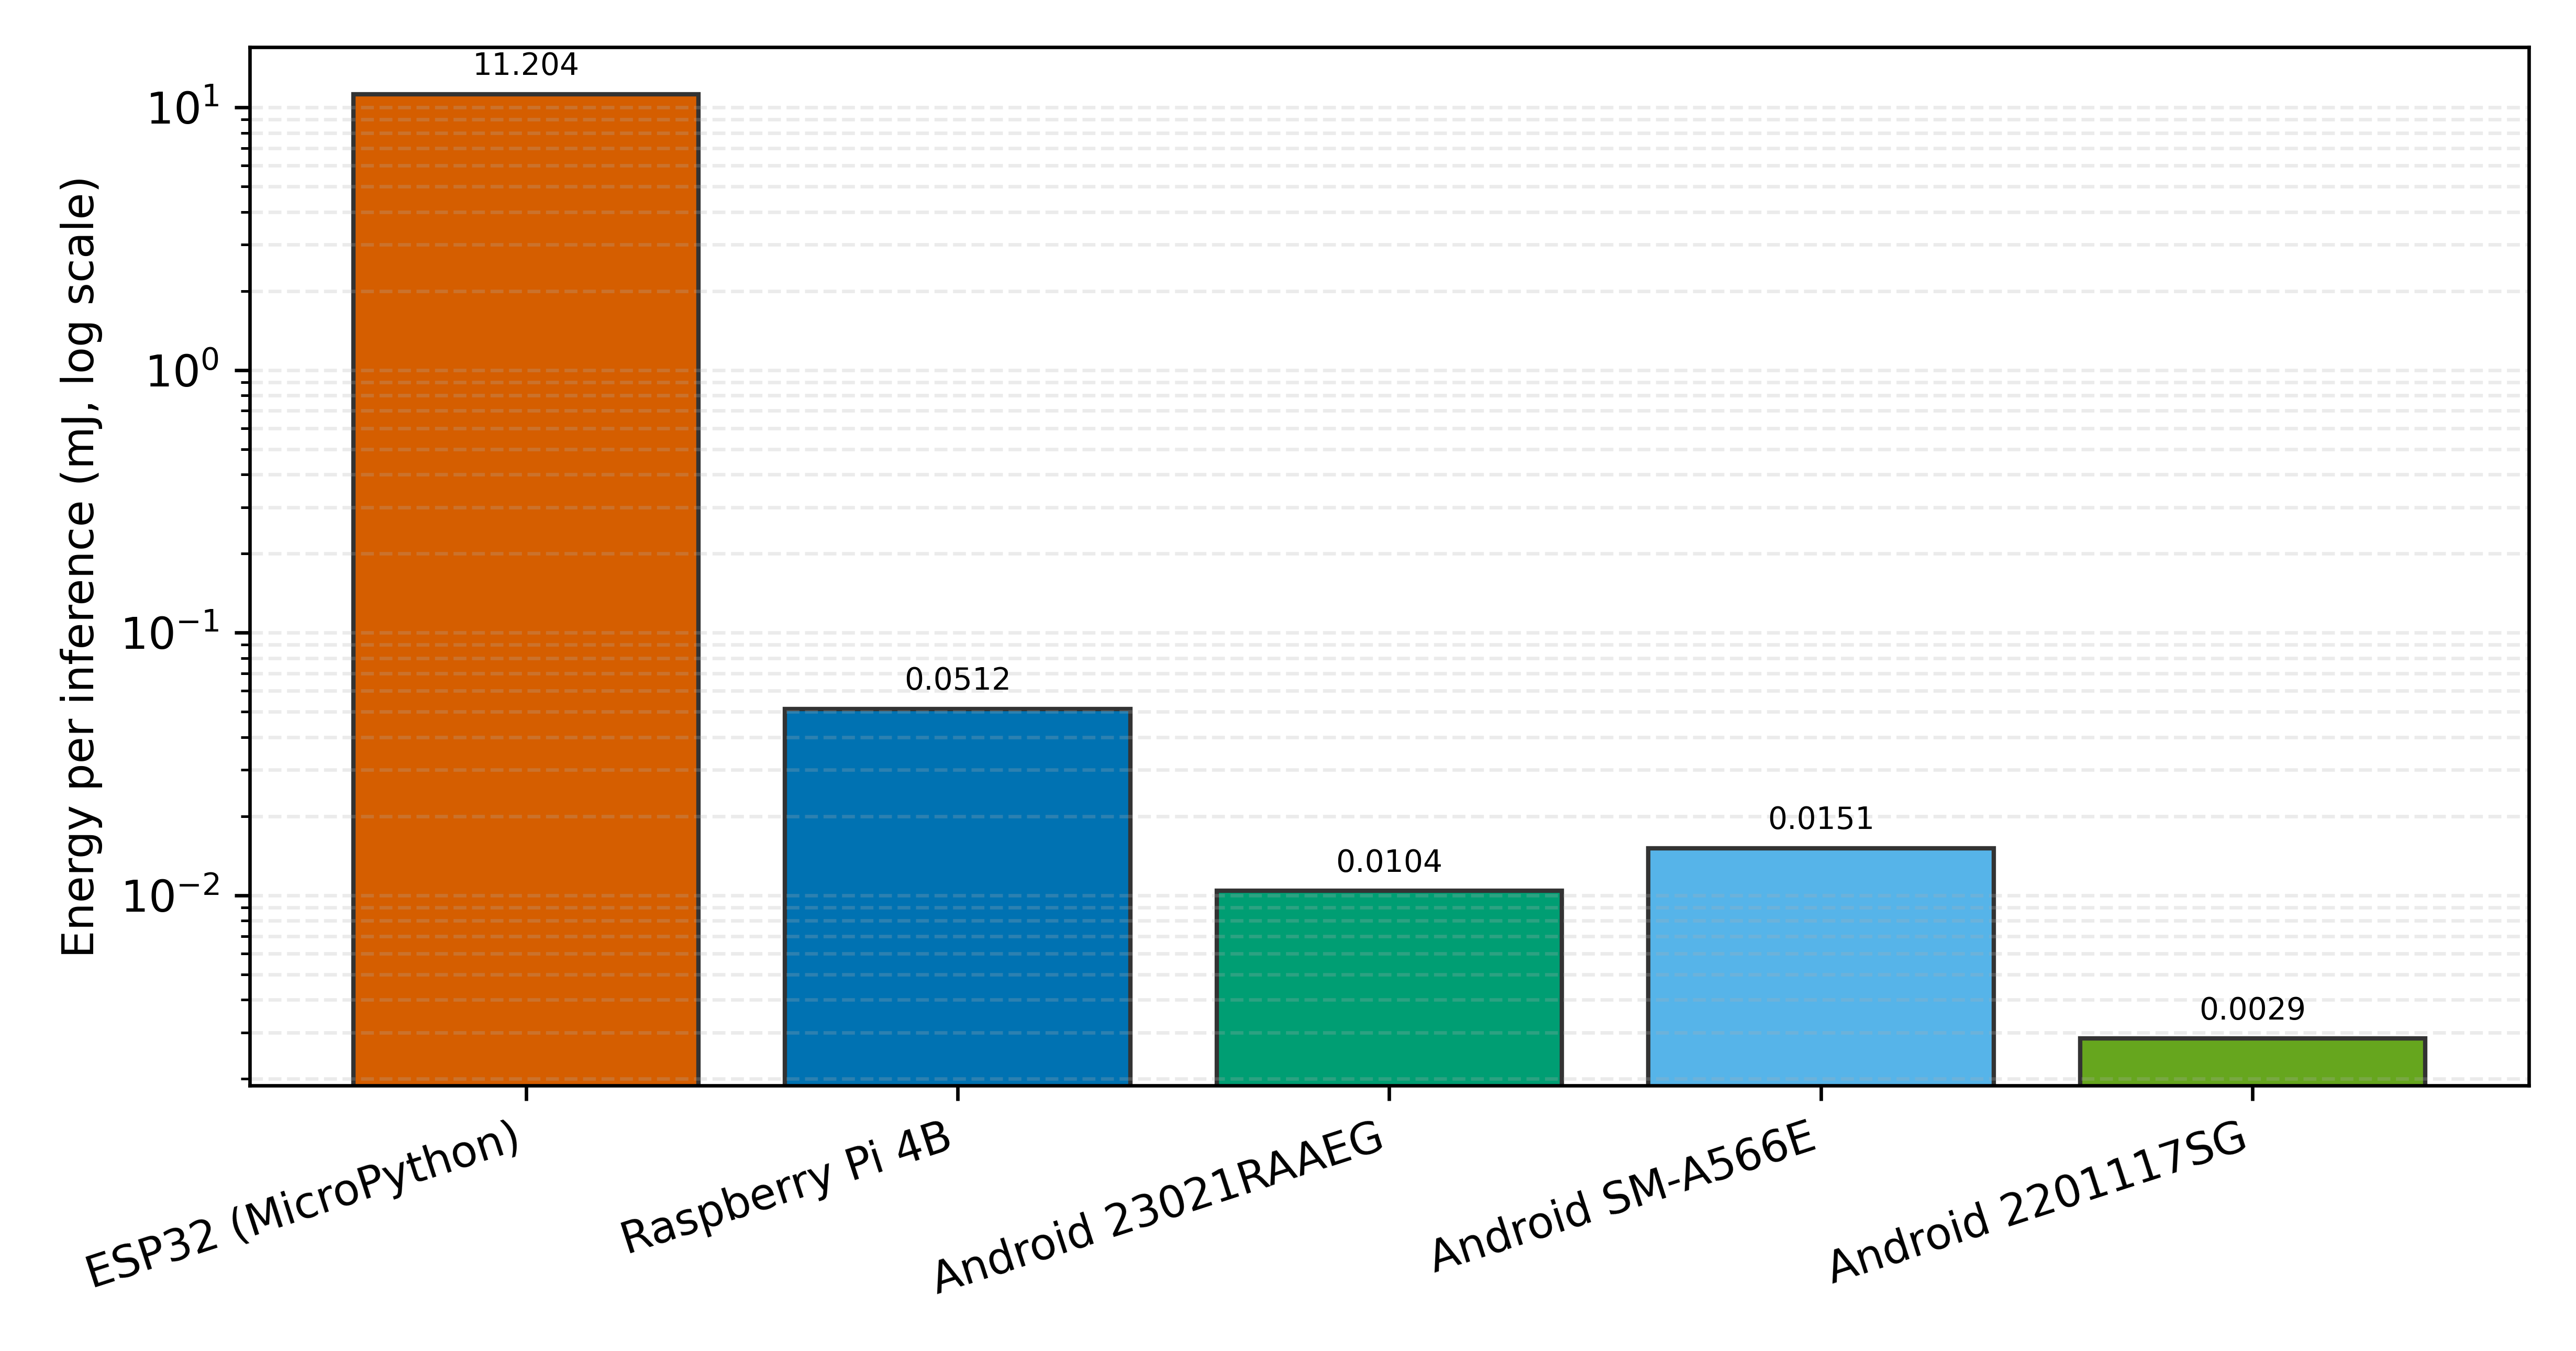
\includegraphics[width=0.82\textwidth]{energy_platforms_bar.png}
\caption{Comparative energy per inference (log scale).}
\label{fig:energy_bar_lnncs}
\end{figure}

Figure~\ref{fig:energy_bar_lnncs} complements Table~\ref{tab:energy_latency} by making the large energy gap between ESP32 and higher-throughput platforms visually explicit on a logarithmic axis. Without log scaling, low-mJ/inf differences among Raspberry Pi and Android devices would be visually compressed; with this scale, relative efficiency differences remain readable and directly comparable.

\FloatBarrier
